\newpage 

\section*{Task 5}
In this section it will be anayzed two particular cases of the TTL AND gate and the CMOS OR gate.
The configurations to analyze are shown below.

\begin{figure}[H]
    \begin{centering}
    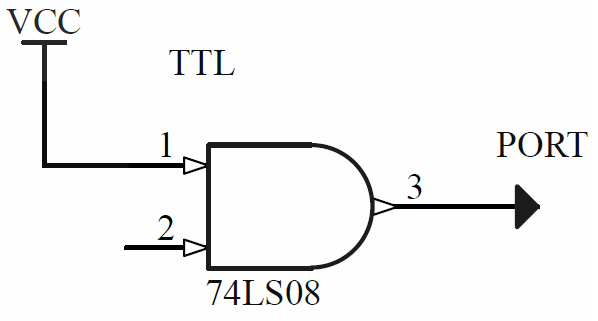
\includegraphics[width=0.3\textwidth]{data/TTL_EJ5}
    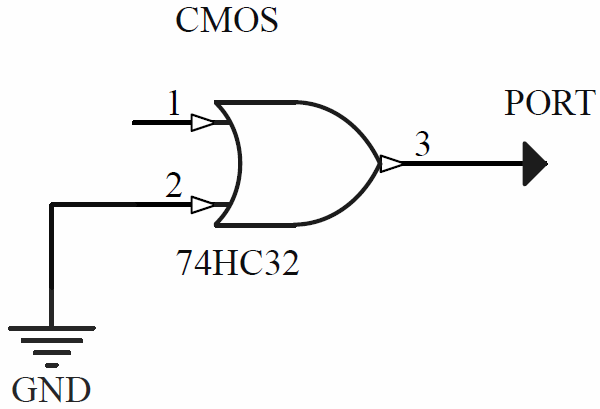
\includegraphics[width=0.3\textwidth]{data/CMOS_EJ5}
    \par\end{centering}
    \caption{TTL AND gate and CMOS OR gate test circuits}
\end{figure}

In the case of the TTL AND gate, with one of the inputs not connected and the other to +VCC,
 the output results on HIGH level. 
That is because the emmiter terminal of the transistor for that input pin is floating without setting 
the potencial to a reference, so the transistor is in cut-off mode, causing that the output 
transistor to be in cut-off mode to, resulting a HIGH level voltage from its colector terminal.

In the case of the CMOS gate, with one of the inputs floating and the other to GND, the output results 
on HIGH level.
That is because the gate terminal of the MOS transistor results floating, without setting the potencial
to a reference, so its not fixed in saturation mode, similar to what happened in the previous case.

Then, both technologies are connected as follows.

\begin{figure}[H]
    \begin{centering}
    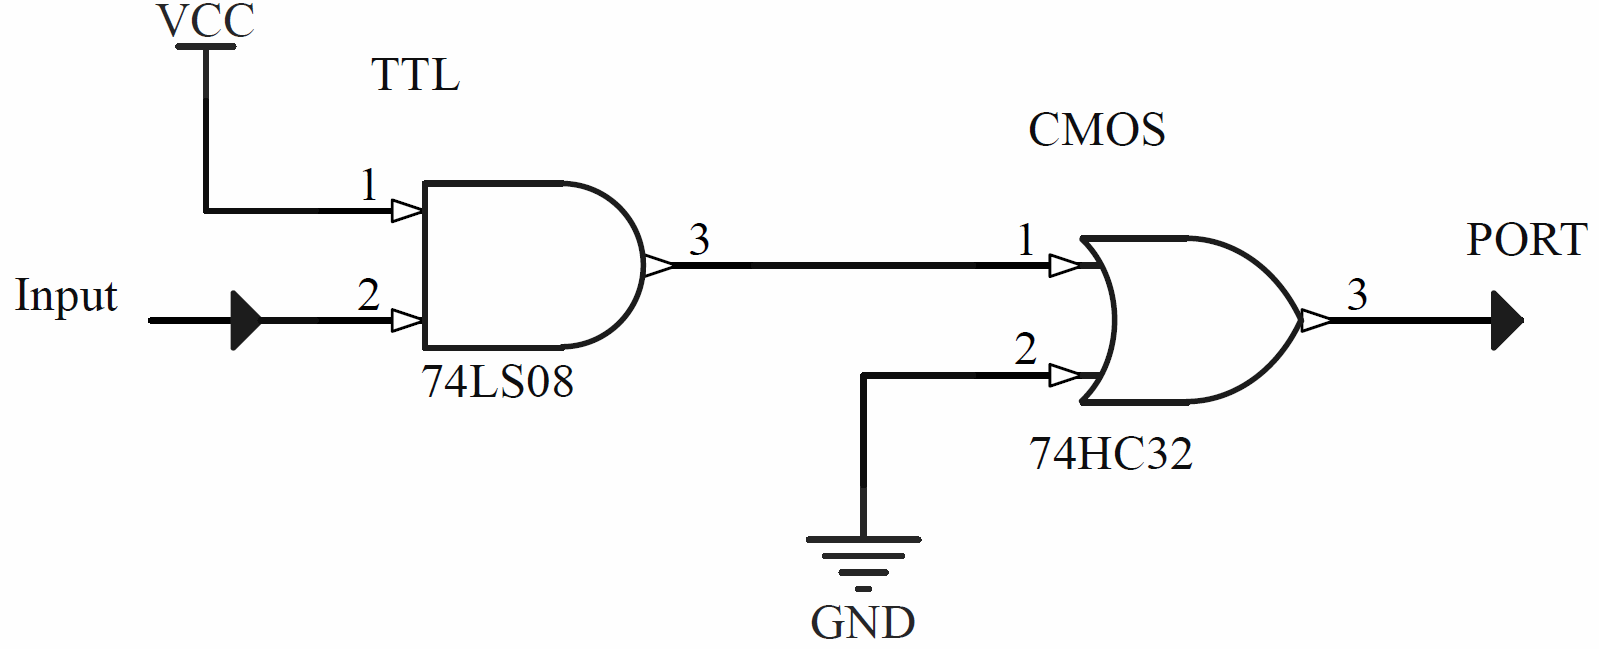
\includegraphics[width=0.7\textwidth]{data/MIX_EJ5}
    \par\end{centering}
    \caption{TTL AND gate and CMOS OR gate connected}
\end{figure}

The problem observed is the same as before: with the input pin floating, the output results on HIGH
level voltage. But this connection has a problem regarding the voltage levels. From the examples used, 
according to Texas Instruments datasheets, 
in 74LS08 for the AND gate the $VOH_{MIN}=2V$ in the worst case and for the 74HC32 (OR gate) the $VIH_{MIN}=3.15V$.
In the worst case, that can cause that although both inputs are in HIGH level, if the AND output is $2V$, 
it will be considered as a $OV$ in the OR gate, showing $0V$ at the final output.
\newpage
The simplest solution may be use both gates from the same technology, but it can be fixed with a 
level shifter circuit, implemented with a PNP transistor as shown below.

\begin{figure}[H]
    \begin{centering}
    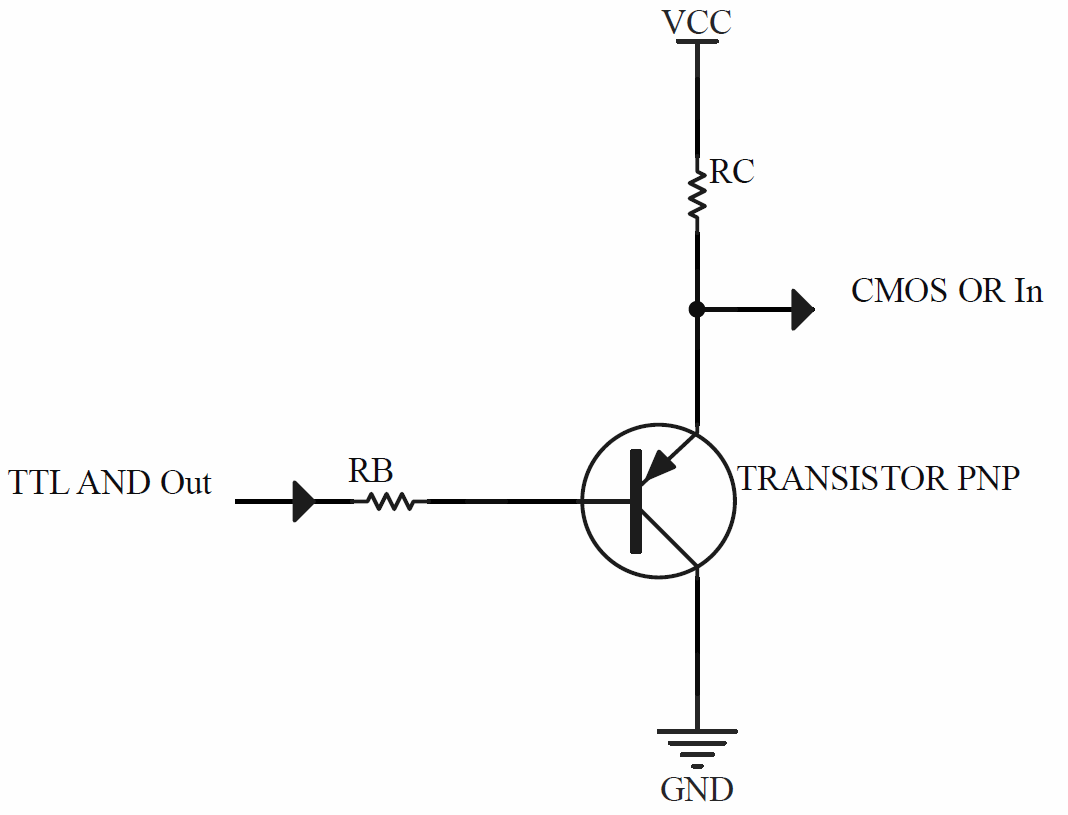
\includegraphics[width=0.4\textwidth]{data/MIXFIX_EJ5}
    \par\end{centering}
    \caption{Level shifter with an PNP transistor}
\end{figure}